\section{AI-Assisted Programming}
To systematically analyze how generative AI influences developer problem-solving, we first characterize the different modes through which developers interact with AI systems during programming tasks. Rather than categorizing tools based on underlying models or capabilities, we focus on interaction patterns that reflect how developers engage with AI assistance in practice. In particular, we distinguish between two primary modes of interaction: exploration and acceleration. Exploration-oriented interactions involve using AI to understand problems, generate ideas, and examine alternative solutions, often through iterative and conversational engagement. In contrast, acceleration-oriented interactions focus on efficiently completing tasks by leveraging AI-generated suggestions or code with minimal deliberation. This distinction provides a useful lens for analyzing how AI support shapes developer behavior across different stages of problem-solving.

\paragraph{Generative AI as an Autocomplete Tool}
When solving structured programming tasks such as those found in Advent of Code \cite{adventOfCode}, developers often decompose the problem into smaller subtasks, such as parsing input into appropriate data structures. Even when the solution approach is clear, generative AI tools can be used to accelerate implementation by assisting with code completion and reducing the effort of recalling syntax or API details. Developers may provide contextual comments to guide the tool, after which inline suggestions appear during pauses in typing. These suggestions, including end-of-line completions (Figure \ref{figure:taxonomy:autocomplete}), enable faster code writing while maintaining the developer's original intent.
\begin{figure}
    \centering
    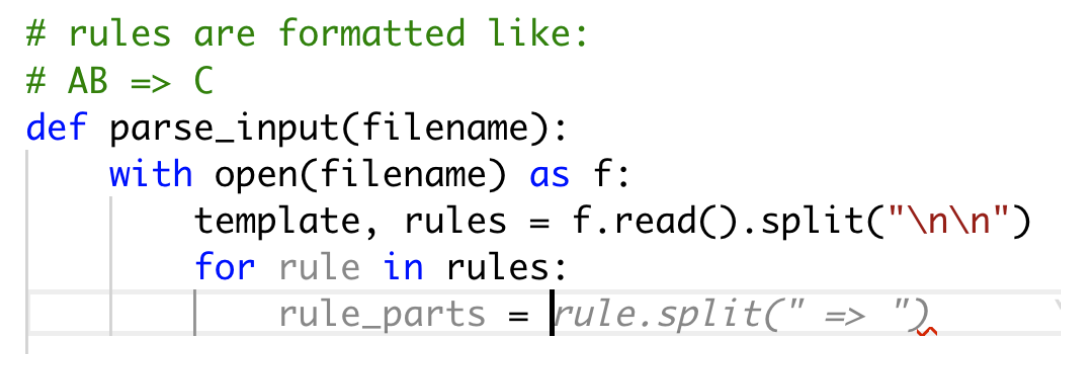
\includegraphics[width=\columnwidth]{content/figures/taxonomy-autocomplete.png}
    \caption{An example of an end-of-line suggestion from Copilot, which completes the current line of code based on the context provided by preceding code and comments.}
    \label{figure:taxonomy:autocomplete}
\end{figure}
In this case (Figure \ref{figure:taxonomy:autocomplete}), Copilot suggests the correct API function invocation to split the rule into its left- and right-hand sides. To come up with this suggestion, Copilot relies on the context, i.e. some amount of source file content preceding the cursor, which can include both code and natural language comments, as is the case in our example.

\paragraph{Generative AI as an Exploration Tool} When developers encounter unfamiliar tasks, generative AI can be used as an exploration tool to understand both the problem and potential solution approaches.
\begin{figure}
    \centering
    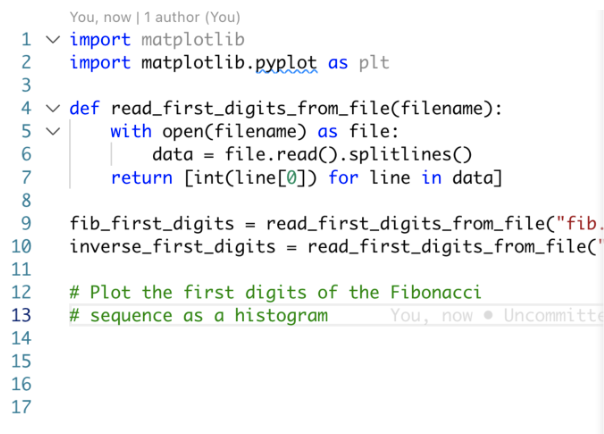
\includegraphics[width=\columnwidth]{content/figures/taxonomy-generation-1.png}
    \caption{Example code where a user needs a more lengthier suggestion}
    \label{figure:taxonomy:generation:1}
\end{figure}
Developers may begin by expressing the task through natural language prompts (lines 12-13 of Figure \ref{figure:taxonomy:generation:1}), which enables the system to generate multiple candidate solutions. By invoking the multi-suggestion interface (Figure \ref{figure:taxonomy:generation:2}), they can examine several alternatives, identify common patterns, and observe relevant API usage, helping build confidence in the generated outputs.
\begin{figure}
    \centering
    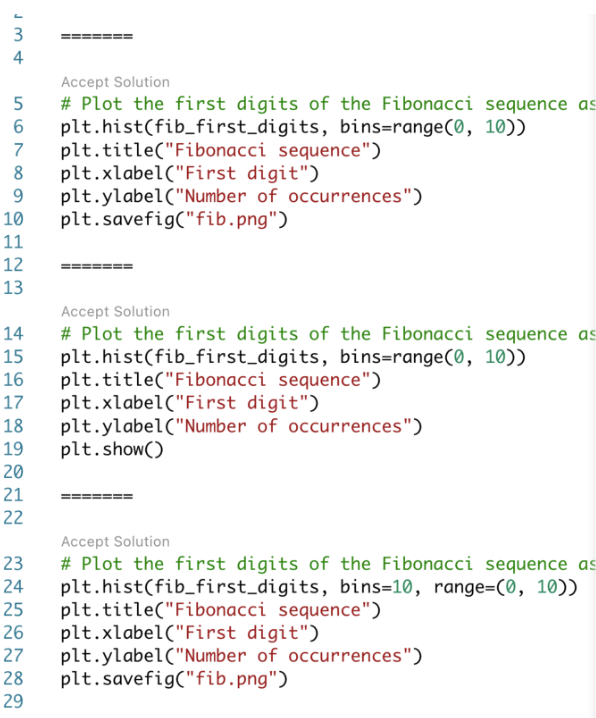
\includegraphics[width=\columnwidth]{content/figures/taxonomy-generation-2.png}
    \caption{An example of Generative AI being used as an exploration tool, where the developer provides a natural language prompt to generate multiple candidate solutions.}
    \label{figure:taxonomy:generation:2}
\end{figure}
This process allows developers to select suitable code snippets while also gaining an understanding of underlying abstractions and libraries. To ensure correctness, the generated code is typically executed and inspected, serving as a form of validation. Such interactions are iterative and deliberate, involving prompt refinement, comparison of alternatives, and verification, reflecting an exploratory mode of problem-solving.

\section{Taxonomy of AI-Assisted Programming}
\subsection{Suggestion-Based Interactions}
Suggestion-based assistance represents a class of AI interactions where developers receive real-time code completions based on the current programming context. These interactions are typically lightweight and minimally intrusive, requiring little to no explicit input beyond the code being written. By providing inline or on-demand suggestions, such systems aim to accelerate implementation by reducing keystrokes, aiding recall of syntax and APIs, and streamlining routine coding tasks. In this section, we categorize suggestion-based assistance into distinct subtypes based on the scope and presentation of generated code.

\subsubsection{End-of-Line Completion}
End-of-line completion represents the most granular form of suggestion-based assistance, where the AI system predicts and completes the remainder of a partially written line of code. These suggestions are typically short, context-aware, and require minimal cognitive overhead to evaluate, enabling developers to maintain flow during implementation. As illustrated in Figure \ref{figure:taxonomy:autocomplete}, such completions often rely on local context and common coding patterns to provide syntactically correct continuations. Prior work shows that developers frequently accept these suggestions due to their low cost of verification and seamless integration into the coding process \cite{barke2022grounded}. This interaction mode primarily reduces keystrokes and supports rapid code construction without significantly altering higher-level problem-solving strategies.

\subsubsection{Multi-Line / Block Completion}
Multi-line or block completion extends suggestion-based assistance by generating larger code segments, such as entire functions, loops, or conditional structures, based on the surrounding context and developer intent. These suggestions provide more substantial acceleration benefits by automating repetitive or boilerplate code generation, allowing developers to focus on higher-level logic. However, larger completions require greater cognitive effort to evaluate and verify, as they may introduce subtle errors or assumptions \cite{vaithilingam2022expectation, kazemitabaar2023copilot}. Studies indicate that while developers benefit from increased productivity, they may also rely on these suggestions without fully understanding the generated code, highlighting a trade-off between efficiency and comprehension \cite{kazemitabaar2023copilot}.

\subsubsection{Context-Aware Pattern Completion}
Context-aware pattern completion refers to suggestions that capture recurring coding patterns or idioms across files or projects, enabling the AI system to generate code that aligns with broader structural or stylistic conventions. These suggestions go beyond local syntax completion by incorporating higher-level contextual signals, such as variable usage, naming conventions, or previously implemented logic. As a result, they can assist in maintaining consistency and reducing redundancy in codebases \cite{raychev2014code}. However, reliance on such patterns may reinforce existing coding habits and limit exploration of alternative implementations, subtly influencing developer decision-making during implementation.

\subsection{Conversational Assistance}
\begin{figure}
    \centering
    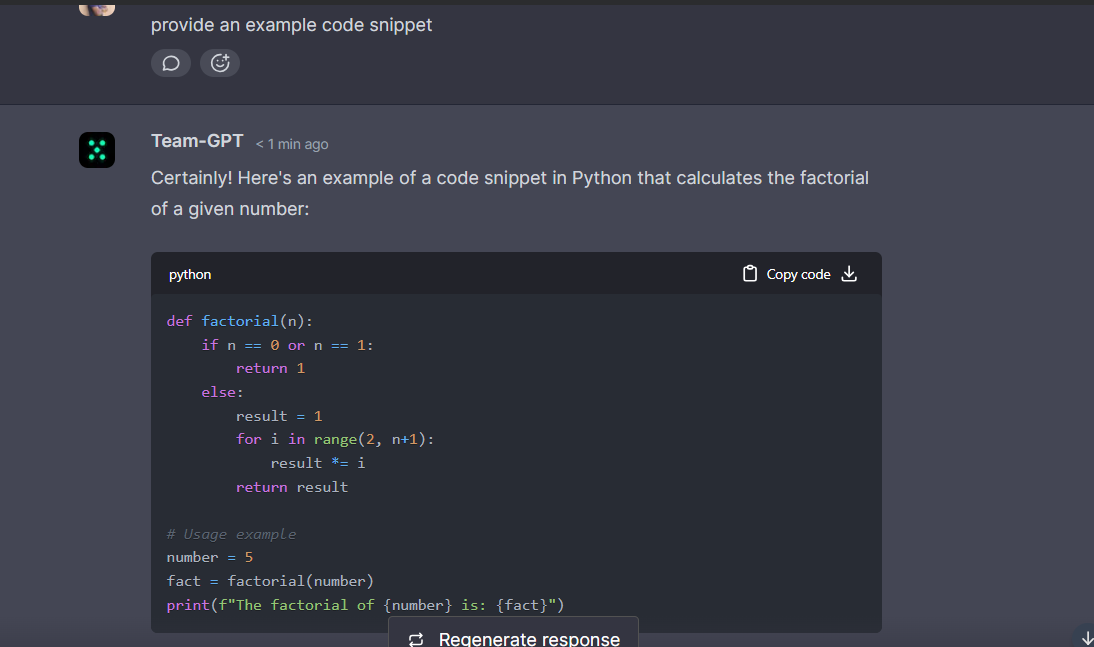
\includegraphics[width=\columnwidth]{content/figures/taxonomy-conversational.png}
    \caption{An example of conversational assistance, where the developer engages in a natural language dialogue with the AI to explore the problem and refine solutions.}
    \label{figure:taxonomy:conversational}
\end{figure}
Conversational assistance refers to interaction modes in which developers engage with generative AI through natural language dialogue (Figure \ref{figure:taxonomy:conversational}) to explore problems, request explanations, or refine solutions \cite{vaithilingam2022expectation, kazemitabaar2023copilot}. Unlike suggestion-based systems, these interactions are explicit and iterative, allowing developers to externalize their reasoning and guide the AI through prompts and follow-up queries. Prior work shows that such conversational workflows enable flexible problem exploration and support tasks such as understanding unfamiliar code, learning APIs, and clarifying requirements.

Conversational assistance can be broadly categorized into query-driven interaction and iterative refinement.
\begin{enumerate}
    \item In \textbf{query-driven interaction}, developers pose direct questions (e.g., requesting explanations or examples), using the AI as an on demand knowledge source.
    \item In \textbf{iterative refinement}, developers progressively adjust prompts based on previous responses, engaging in a back-and-forth dialogue to converge on a desired solution.
\end{enumerate}
These subcategories support exploration-oriented\footnote{Exploration-oriented workflows involve using AI to iteratively explore, compare, and understand multiple solution possibilities before implementation.} workflows by enabling developers to decompose problems, compare alternatives, and refine their understanding, although the quality of outcomes depends heavily on prompt formulation and interpretation \cite{barke2022grounded}.

\subsection{Generative / Transformational Assistance}
\begin{figure}
    \centering
    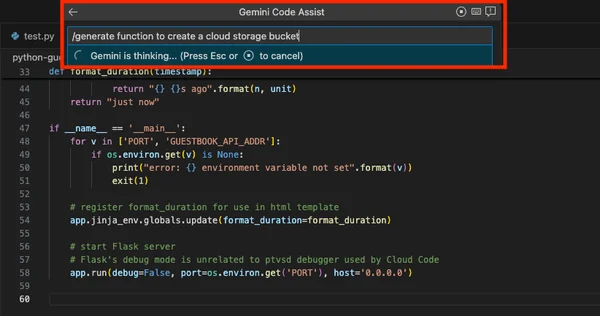
\includegraphics[width=\columnwidth]{content/figures/taxonomy-generation.png}
    \caption{An example of generative assistance, where the developer provides a high-level intent and receives a substantial code output that implements the desired functionality.}
    \label{figure:taxonomy:generation}
\end{figure}
Generative or transformational assistance refers to interaction modes where developers provide high-level intent and receive substantial code outputs, such as functions, program fragments, or refactored implementations. These interactions abstract away low-level details, allowing developers to focus on specifying desired functionality while the AI produces corresponding code artifacts (Figure \ref{figure:taxonomy:generation}). Such capabilities are central to modern LLM-based tools and are widely used to accelerate implementation and reduce manual coding effort \cite{peng2023copilot, kazemitabaar2023copilot}.

This form of assistance can be divided into code generation and code transformation. Code generation involves producing new code from natural language descriptions or partial context, while code transformation focuses on modifying existing code, such as refactoring, optimizing, or fixing bugs. Both subcategories provide significant efficiency gains but require careful validation, as generated outputs may introduce incorrect assumptions or incomplete logic. Studies indicate that developers often rely on these outputs for rapid progress, sometimes at the cost of reduced engagement with underlying problem details \cite{vaithilingam2022expectation, barke2022grounded}.

\subsection{Retrieval and Explanation Assistance}
Retrieval and explanation assistance encompasses interaction modes where generative AI is used to access, summarize, or explain information relevant to programming tasks. Rather than generating new code directly, these interactions focus on supporting comprehension and decision-making by providing contextual knowledge, such as documentation summaries, error explanations, or conceptual clarifications \cite{rasheed2025aireview}. This mode aligns closely with traditional information retrieval tasks but benefits from the contextual reasoning capabilities of LLMs \cite{nguyen2025genai}.

This category can be divided into information retrieval and code explanation.
\begin{enumerate}
    \item \textbf{Information retrieval} involves locating and summarizing relevant documentation or examples, reducing the need for manual search.
    \item \textbf{Code explanation} focuses on interpreting existing code, errors, or outputs to help developers understand behavior and identify issues.
\end{enumerate}
These subcategories are particularly valuable during debugging and learning phases, as they reduce cognitive overhead associated with searching and interpreting external resources. However, reliance on AI-generated explanations may affect how developers internalize knowledge and reason about code correctness \cite{kazemitabaar2023copilot}.

\section{Connection of these terms with Software Development Process}
The adoption of generative AI tools in software engineering has accelerated significantly, with developers increasingly incorporating systems such as code generation assistants and conversational agents into their workflows. Large-scale studies and surveys indicate that AI-assisted programming tools are now commonly used for tasks ranging from code synthesis to debugging and learning \cite{nijkamp2022codegen, li2023competition}. These tools are no longer peripheral utilities but are becoming embedded components of modern development environments, influencing how developers structure and execute programming tasks.

The interaction modes introduced by generative AI systems, as captured by the taxonomy presented earlier, exhibit distinct relationships with different stages of the software development process. Prior work has highlighted that developer-AI interaction is not uniform, but varies based on task context, intent, and level of abstraction \cite{mohammadkhani2023systematic, crawford2023aisesurvey}. By mapping suggestion-based, conversational, generative, and retrieval-oriented assistance to development stages, we can better understand how these tools shape problem-solving strategies and workflow dynamics.

Conversational assistance is most closely associated with the ideation stage, where developers engage in problem understanding, requirement clarification\footnote{Here, we refer to the individual developer solving a problem, excluding Software Development Models, eg, Waterfall, Agile, etc.}, and exploration of potential solutions. Natural language interaction enables developers to iteratively refine their understanding and query the system for explanations, examples, and alternative approaches. Such interactions support exploratory reasoning and have been shown to facilitate learning and problem decomposition, particularly in unfamiliar domains \cite{yang2025llmworkflows, crawford2023aisesurvey}.

Suggestion-based and generative assistance primarily influence the development stage, where ideas are translated into executable code. Suggestion-based tools provide fine-grained completions that reduce the effort of writing syntactically correct code, while generative systems can produce larger functional units or transformations from high-level intent. These capabilities significantly accelerate implementation, allowing developers to focus on higher-level design decisions, although they may also introduce challenges related to verification and understanding \cite{nijkamp2022codegen, li2023competition}.

Retrieval and explanation assistance play an important role in the review stage, supporting debugging, validation, and reasoning about program behavior. By summarizing documentation, explaining errors, and interpreting code, these tools reduce the cognitive burden associated with information retrieval and comprehension. This enables developers to more efficiently identify issues and validate correctness, particularly in complex or unfamiliar codebases \cite{mohammadkhani2023systematic}.

Finally, conversational and generative assistance extend into the documentation stage, where developers generate or refine descriptions of code, usage instructions, and comments. These tools can synthesize documentation directly from code or assist in rephrasing and structuring explanations through iterative interaction. As a result, they help streamline documentation practices \cite{yang2025llmworkflows} and improve consistency, further integrating AI support across the development lifecycle.

In the following section, we examine each of these development stages in detail, providing a deeper analysis of how generative AI influences developer behavior and problem-solving strategies within each stage.